\documentclass[a4paper]{article}


\usepackage{alphabeta} 
\usepackage{enumitem} 
\usepackage{mathtools}
\usepackage{amsmath, amssymb} 
\usepackage{amsthm}
\usepackage{cancel} 
\usepackage[margin=0.70in]{geometry} 
\geometry{left=3cm,right=3cm,top=2.8cm,bottom=3cm}	%the page geometry as defined, A4=210x297mm
\usepackage{graphicx}
\usepackage{wrapfig}
\usepackage{caption}
\usepackage{textcomp}
\usepackage{tabto}
\usepackage{layout}
\usepackage{bm}
\usepackage{minipage-marginpar}
\usepackage[dvipsnames]{xcolor}
\usepackage{hyperref}
\usepackage{dutchcal}
\usepackage{derivative}
\usepackage{esint}
%\usepackage{biblatex}
\usepackage{subcaption}
\usepackage{booktabs}\usepackage{derivative}
\usepackage[flushleft]{threeparttable}
\usepackage[capbesideposition=outside,capbesidesep=quad]{floatrow}


%%RENEW

\newtheorem{problem}{Άσκηση}
\newtheorem*{solution*}{Λύση}
\newtheorem{definition}{Ορισμός}[subsection]
\newtheorem{properties}{Ιδιότητες}[subsection]
\newtheorem{theorem}{Θεώρημα}[subsection]
\newtheorem{protash}{Πρόταση}[subsection]
\newtheorem{porisma}{Πόρισμα}[subsection]
\newtheorem{lemma}{Λήμμα}[subsection]
\newtheorem*{prooof}{Απόδειξη}
\newtheorem*{notes}{Παρατηρήσεις}
\newtheorem*{note}{Παρατήρηση}
\newtheorem*{app}{Εφαρμογή} 
\newtheorem*{example}{Παράδειγμα}
\newtheorem*{examples}{Παραδείγματα}

%\renewcommand{\labelenumi}{\roman{enumi}}
\newcommand{\approxtext}[1]{\ensuremath{\stackrel{\text{#1}}{\approx}}}
\renewcommand{\figurename}{Εικόνα.}
\renewcommand{\tablename}{Πίνακας.}
%\renewcommand\refname{New References Header}
\renewcommand*\contentsname{Περιεχόμενα}

\begin{document}
\begin{titlepage}			%makes a title page. Remember to change the author, CID, username and group number to what is appropriate for you!
	\centering
	{\scshape\LARGE Εθινικό Μετσόβιο Πολυτεχνείο\par}
	{\scshape \LARGE Σ.Ε.Μ.Φ.Ε.\par}
	\vspace{1cm}
	{\huge\bfseries Εξισώσεις Fresnel\par}
	\vspace{1cm}
	{\Large\itshape Θωμόπουλος Σπύρος\par}		%remember to change these!
	
	%		{\large Group \@group\unskip\strut\par}
	{\large A.M ge19042 \hfill \\}% spyros.thomop@gmail.com/ ge19042@mail.ntua.gr\par		%remember to change these!
	\vspace{1cm}
	{\large 25/10/2021\par}
\end{titlepage}


\newpage 

\subsection*{Σκοπός}
Ο στόχος της εν λόγω εργαστηριακής άσκησης είναι να μελετηθεί η ανάκλαση του γραμμικά πολωμένου φωτός σε επίπεδη επιφάνεια διηλεκτρικού. Συγκεκριμένα θα εξεταστεί η ένταση της δέσμης όταν είναι πολωμένη παράλληλα στο επίπεδο πρόσπτωσης-ανάκλασης και όταν βρίσκεται σε μία ενδιάμεση γωνία.
\subsection*{Θεωρητικά Στοιχεία}
Ένα Η/Μ κύμα αποτελείται από ένα ηλεκτρικό$ (\vec{E})$ και ένα μαγνητικό $(\vec{B})$ πεδίο που ταλαντώνονται κάθετα μεταξύ τους και κάθετα στη διεύθυνση διάδοσης (εγκάρσιο κύμα). Ορίζουμε ως διεύθυνση πόλωσης του κύματος την διεύθυνση ταλάντωσης του ηλεκτρικού πεδίου.

Όταν ένα Η/Μ κύμα περνάει από ένα διηλεκτρικό υλικό σε ένα άλλο μέσω μίας επίπεδης επιφάνειας, τότε ανεξαρτήτως της πόλωσής του ισχύουν οι παρακάτω νόμοι: 


\begin{itemize}
\item[.] $\theta_{in} = \theta_r$,\hspace{1cm} όπου $\theta_{in}, \theta_r$ οι γωνίες πρόσπτωσης και ανάκλασης
\item[.] $n_1 sin\theta_{in} = n_2 sin\theta_t$,\hspace{0.3cm} όπου $n_1, n_2$ οι δείκτες διάθλασης του κάθε μέσου και $\theta_t$ η γωνία  

			\hspace{3.35cm} διάθλασης (ν. Snell).
\end{itemize}

Γενικά μας ενδιαφέρει η μεταβολή της έντασης (μέση ισχύς ανά μονάδα επιφάνειας) του Η/Μ κύματος κατά την διάθλαση και την ανάκλασή του. Στην πρώτη φάση του πειράματος μελετάμε την π-πόλωση (επίπεδο πόλωσης $\parallel$ επίπεδο ανάκλασης-διάθλασης). \footnotemark
\footnotetext{Υπάρχει και η περίπτωση της σ-πόλωσης στην οποία ίσχύει ότι επίπεδο πόλωσης $\perp$ επίπεδο ανάκλασης-διάθλασης για την οποία αλλάζουν οι εξισώσεις Fresnel, η οποία δεν μελετήθηκε.}
 Εδώ τα πεδία $\vec{B}$ και $\vec{H}$ εφάπτονται της διαχωριστικής επιφάνειας ενώ τα $\vec{E}$ και $\vec{D}$ είναι κάθετα σ' αυτή. Έπειτα από την εφαρμογή των συνοριακών συνθηκών προκύπτουν οι εξισώσεις Fresnel για τους συντελεστές ανάκλασης και διέλευσης πλάτους
\begin{equation}\label{1}
 r_{\parallel} := \left( \frac{E_r}{E_{in}} \right)_{\parallel} = \frac{n_2cos\theta_{in}-n_1cos			              \theta_t}{n_2cos\theta_{in}+n_1cos\theta_t}     
 \end{equation}
 
 \begin{equation}\label{2}
	t_{\parallel} := \left( \frac{E_t}{E_{in}} \right)_{\parallel} = \frac{2n_1cos\theta_{in}}{n_2cos\theta_{in}+n_1cos\theta_t}
\end{equation}
	
Παρατηρούμε πως αν $\theta_{in} + \theta_{t} = \pi/2$ τότε $\theta_{t} = 0 $, ο συντελεστής ανάκλασης μηδενίζεται για μία συγκεκριμένη γωνία πρόσπτωσης η οποία καλείται γωνία Brewster και υπολογίζεται από την σχέση: 

\begin{equation}\label{3}
 tan\theta_{B} = n_2/n_1 
\end{equation}
	όπου για εμάς το μέσο 1 θα είναι αέρας, άρα $n_1=1$ και $n_2=n_{πρισματος} = n$.
	
	Ορίζονται ακόμη συντελεστές διέλευσης και διάδοσης της έντασης του κύματος 
	\begin{equation}\label{4}
	R := \frac{I_r}{I_{in}} = \left( \frac{E_r}{E_{in}} \right)_{\parallel}^2 = r_{\parallel}^2
	\end{equation}
	 
	 \begin{equation}\label{5}
	 	 T := \frac{n_2 cos\theta_{t}}{n_1cos\theta_{in}} \frac{I_t}{I_{in}} = \frac{n_2 cos\theta_{t}}{n_1cos\theta_{in}}  \left( \frac{E_t}{E_{in}} \right)_{\parallel}^2 = \frac{n_2 cos\theta_{t}}{n_1cos\theta_{in}}  t_{\parallel}^2 
	 \end{equation}
με την χρήση των οποίων μπορεί να εκφραστεί η Αρχή Διατήρησης της Ενέργειας 
	$$T_{\parallel} + R_{\parallel} = 1 $$

Γενικά, ενδέχεται το επίπεδο πόλωσης του κύματος να μην είναι παράλληλο στο επίπεδο ανάκλασης-διάθλασης, αλλά αποκλίνει κατά μία γωνία $\delta$. Σε αυτή τη περίπτωση η ανακλώμενη δέσμη είναι πολωμένη σε μία διαφορετική γωνία $\omega$ για την οποία ισχύει 
$$ tan\omega = - \frac{sin(\theta_{in}-\theta_{t})}{sin(\theta_{in}+\theta_{t})} \cdot \frac{tan(\theta_{in}-\theta_{t})}{tan(\theta_{in}+\theta_t)} tan\delta $$
και στην περίπτωση που το πρώτο διηλεκτρικό είναι ο αέρας ($n_1=1$), το δεύτερο έχει δείκτη διάθλασης $n_2 = n$ και η γωνία απόκλισης της πόλωσης της προσπίπτουσας δέσμης είναι $\delta=\pi/4$ έχουμε: 
 
\begin{equation}\label{6}
\Psi := \delta - \omega = Arctan\left( - \frac{cos\theta_{in}\sqrt{n^2-sin^2\theta_{in}}}{sin^2\theta_{in}} \right)  
\end{equation}

 Ακόμη αν η στροφή του επιπέδου πόλωσης της ανακλώμενης δέσμης γίνει $\Psi=\pi /4$ τότε έχουμε 
 

%\begin{equation}
  \begin{align*}
% \begin{mulitlined}
 	1 =-  \frac{cos\theta_{in}\sqrt{n^2-sin^2\theta_{in}}}{sin^2\theta_{in}} \Rightarrow -tan\theta_{in}sin\theta_{in} = \sqrt{n^2-sin^2\theta_{in}} \Rightarrow  \end{align*} 
 	
 	\begin{align}\label{7} 
 	 n^2 = sin^2\theta_{in} \left( tan^2\theta_{in} + 1  \right) \Rightarrow \boxed{n = tan\theta_{in} }
 	\end{align}
 %\end{multilined}

%  \end{equation}

 όπου μπορούμε να μετρήσουμε την γωνία πρόσπτωσης $\theta_{in}$, άρα κσι με αυτή τη μέθοδο γίνεται εφικτός ο πειραματικός προσδιορισμός του δείκτη διάθλασης.
 
 
 
\subsection*{Πειραματική Διάταξη}

Η πειραματική διάταξη αποτελείται από: 

%\begin{minipage}[l!]{0.5\textwidth}\raggedleft
\begin{itemize}

\item[.] Laser He-Ne 1.0mW, 220V AC, πολωμένο παράλληλα στην ενδεικτική λυχνία
\item[.] 2 πολωτικά φίλτρα με βαθμονόμηση 
\item[.] Ισοσκελές τριγωνικό πρίσμα από πυριτύαλο 60 μοιρών
\item[.] Οπτική τράπεζα με στρήριγμα για το πρίσμα 
\item[.] Φωτοανιχνευτή (Μετατρέπει την ένταση της δέσμης σε συνεχές ηλετρικό ρεύμα) 
\item[.] Αναλογικό πολύμετρο με ενισχυτή 
\item[.] Μηχανισμός στήριξης της διάταξης ( αρθωτό γωνιακό στήριγμα, κύλινδρος στήριξης, βάσεις τύπου τρίποδα, 					στηρίγματα ορθής γωνίας, τετραγωνικές ράβδοι στήριξης) 
\end{itemize}

%\end{minipage}
\hfill 

%\begin{minipage}[r!]{0.5\textwidth}\raggedright
	\begin{figure}[h!]
		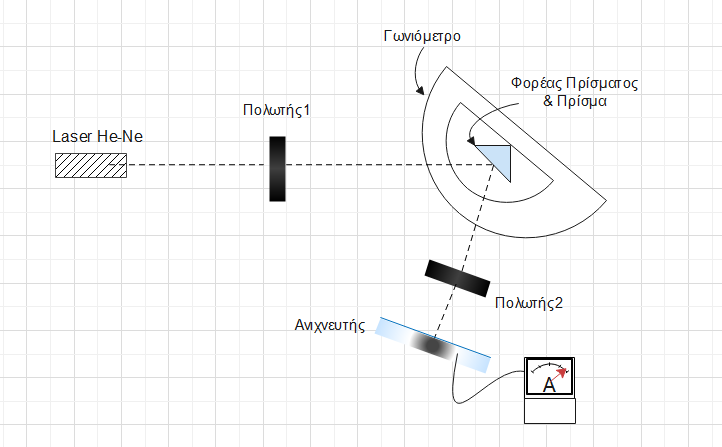
\includegraphics[scale=0.4]{setup.png}
	\end{figure}
%\end{minipage}



\subsection*{Πειραματική Διαδικασία - Επεξεργασία Μετρήσεων}

\subsubsection*{1$^o$ Μέρος (π-πόλωση)}
Αρχικά συναρμολογούμε την διάταξη χρησιμοποιώντας μόνο τον Πολωτή 1, με γωνία πόλωσης $90^o$, δηλαδή η εξερχόμενη δέσμη είναι οριζόντια πολωμένη. Φροντίζουμε η δέσμη να διέρχεται μέσω του πολωτή, περίπου στο μέσο του πρίσματος και προφανώς να πέφτει στον ανιχνευτή. Ρυθμίζουμε το γωνιόμετρο έτσι ώστε η ανακλώμενη δέσμη όταν προσπίπτει κάθετα στο πρίσμα να επιστρέφει στο σημείο εκπομπής της και σημειώνουμε ότι η εν λόγω γωνία είναι $\theta_0 = (0\pm 1)^o$.
% και παρατηρούμε πως η γωνία αναφοράς της κλίμακας είναι. 

Σε πρώτη φάση πρέπει να προσδιορίσουμε την γωνία Brewster προκειμένου να υπολογίσουμε τον δείκτη διάθλασης του γυαλιού από την σχέση  (\ref{3}). Περιστρέφοντας το γωνιόμετρο, παρατηρούμε πως η ένταση της ανακλώμενης δέσμης μηδενίζεται (στην μέτρηση δεν μηδενίζεται, απλώς είναι η ελάχιστη που ανιχνέυσαμε $I_{min}=(0.1\pm0.04)\mu A$ ) για γωνία 
$$ \theta_B = (60\pm1)^o$$
Άρα έχουμε: 
$$n = (1.732 \pm 0.070 ) \footnotemark$$

\footnotetext{Το σφάλμα του δείκτη διάθλασης πρκύπτει απ' τη διάδοση του σφάλματος της γωνίας Brewster 
$$ \delta n = \sqrt{\left( \pdv{n}{\theta_B} \delta\theta_B\right)^2 }=\left| \frac{1}{cos^2\theta_B}\underbrace{\delta\theta_B}_{rad}  \right| = 0.069814$$ }


Τώρα μετράμε την ένταση του ρεύματος που ανιχνεύει το πολύμετρο καθώς μεταβάλλουμε την γωνία πρόσπτωσης (περιστρέφοντας το γωνιόμετρο) με τιμές στο διάστημα $15-80^o$ με βήμα $5^o$.\footnote{Η ένδεξη στο αμπερόμετρο πρέπει να καταγράφεται όταν η ένδειξη φτάνει στο μέγιστο.}
Οι μετρήσεις φαίνονται στον Πίνακα Ι. \footnotemark

\footnotetext{Το σφάλμα του πολυμέτρου στην μέτρηση του ρεύματος εξαρτάται από την κλίμακα στην οποία βρισκόμαστε, 
$$ \delta I = 1.5\% \times \text{κλίμακα} + \text{Σφάλμα ανάγνωσης}$$ όπου το σφάλμα ανάγνωσης ισούται με την ελάχιστη υποδιαίρεση της εκάστοτε κλίμακας, άρα $\delta I_1=0.04, \delta I_3=0.15, \delta I_{10} = 0.4$}


%Ακόμη, στον Πίνακα Ι φαίνονται οι τιμές για την γωνία διάθλασης που δίνονται απ' τον νόμο του Snell\footnotemark, η τιμή του συντελεστή ανάκλασης πλάτους r, η τιμή του συντελεστή ανάκλασης R για κάθε γωνία πρόσπτωσης, βήματα τα οποία έχουν σκοπό τον υπολογισμό της θεωρητικής τιμής της έντασης του ανακλώμενου φωτός.\footnotemark
 Η ένταση της προσπίπτουσας δέσμης είναι $I_{in} = 30\mu A$ και δεν επηρεάζεται από την παρουσία του πολωτή σύμφωνα με τον νόμό του Malus $I'_{in}=I_{in} cos(0) = I_{in} = 30\mu A$
%\footnotetext{$\theta_t = Arcsin\frac{sin\theta_{in}}{n}$}
%\footnotetext{Η ένταση της δέσμης είναι ανάλογη με το τετράγωνο του ηλεκτρικού πεδίου της, άρα μπορεί να χρησιμοποιηθεί η σχέση (\ref{1}) για τον συντελεστή ανάκλασης πλάτους.}

\begin{table}[h!]
	\centering
	\caption{Γραφική παράσταση $I=I(\theta_{in})$}
\begin{tabular}{r|r|r|r}%||r|r|r|r}
$\theta_{in}(\pm1^o)$ & $I_{πειρ}$ & Κλίμακα στο &  $\delta I$ \\%& $\theta_t(^o)$ & r & R & $I_{θεωρ}$\\ 
& $(\mu A)$&  αμπερόμετρο & $(\mu A)$\\    % & & & & $(\mu A)$ \\ 
\hline\hline 
15 &        2.5 &       3 & 0.15 \\%& 8.5941 &    0.2571 & 0.0661\\        
20 &        2.3 &       3 & 0.15 \\%& 11.3891 &   0.2482 & 0.0616\\
25 &        2.2 &       3 & 0.15\\ %& 14.1231 &   0.2362 & 0.0558\\               
30 &        2.1 &       3 & 0.15 \\%& 16.7792 &   0.2208 & 0.0487\\               
35 &        1.7 &       3 & 0.15 \\%& 19.3395 &   0.2012 & 0.0405\\              
 40 &        1.2 &       3 & 0.15 \\%& 21.7850 &  0.1766 & 0.0312\\               
 45 &        0.8 &       3 & 0.15 \\%& 24.0956 &  0.1459 & 0.0213\\               
 50 &        0.5 &       3 & 0.15 \\%& 26.2500 &  0.1077 & 0.0116\\               
 55 &        0.2 &       1 & 0.04 \\%& 28.2261 &  0.0599 & 0.0036\\               
 60 &        0.1 &       1 & 0.04 \\%& 30.0010 &  -0.0000 & 0.0000\\               
 65 &        0.7 &       1 & 0.04 \\%& 31.5520 &  -0.0759 & 0.0058\\               
 70 &        1.1 &       1 & 0.04 \\%& 32.8572 &  -0.1729 & 0.0299\\              
 75 &        3.2 &      10 & 0.40 \\%& 33.8965 &  -0.2987  &0.0892\\               
 80 &        9.1 &      10 & 0.40 \\%& 34.6524 &  -0.4645 &0.2158\\ 
 
                           
 \end{tabular}
\end{table}



Γραφικά,η θεωρητική και η πειραματική καμπύλη της έντασης του του ανακλώμενου φωτός συναρτήσει της γωνίας πρόσπτωσης φαίνεται στην Εικόνα. 1. Η συνάρτηση για τη θεωρητική τιμή της έντασης της ανακλώμενης δέσμης, $I_{th} = I_{th}(\theta_{in})$, προκύπτει από την σχέση (\ref{4}) αντικαθιστώντας από τον ν. Snell $\theta_t = Arcsin\frac{sin\theta_{in}}{n}$
\begin{figure}[h!]
\centering 
\caption{ }
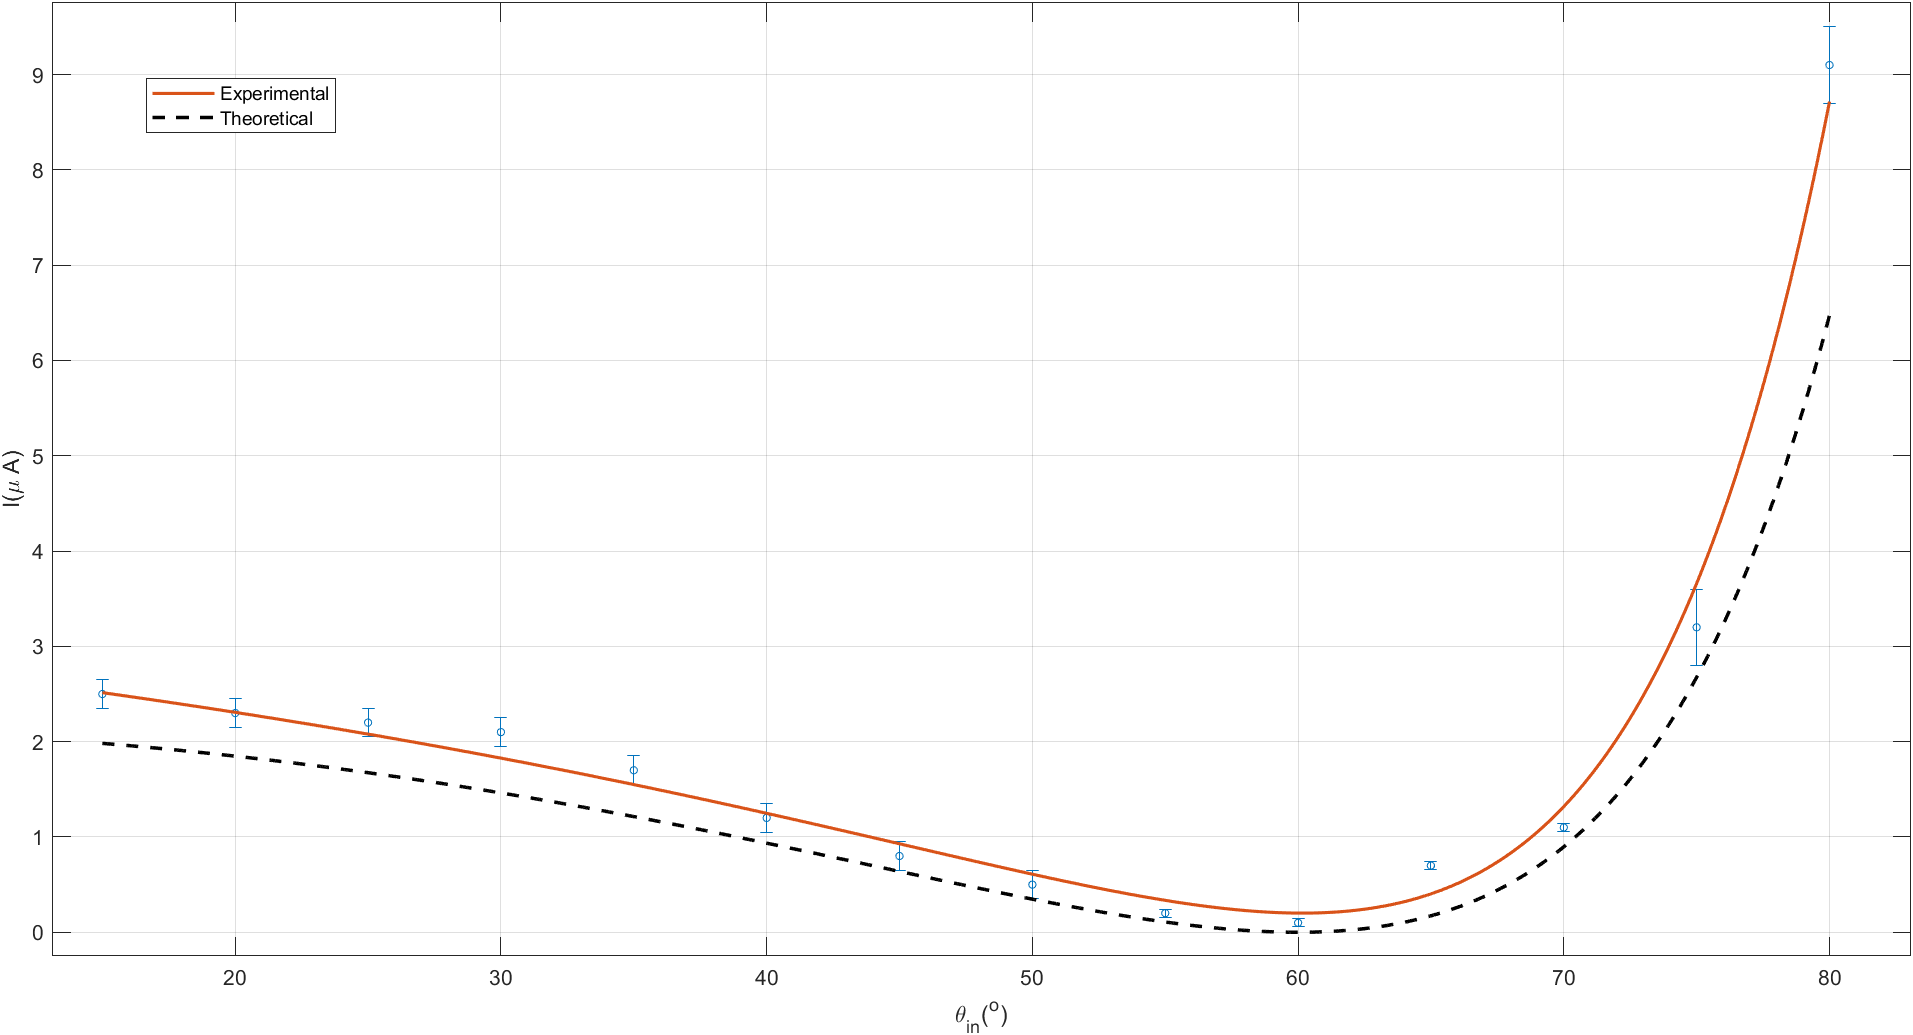
\includegraphics[scale=0.5]{I(th).png}
\end{figure}
 \\ \\
Παρατηρώ ότι οι δύο γραφικές παραστάσεις έχουν την ίδια μορφή, λαμβάνοντας ελάχιστο στην περιοχή των $60^o$. Ωστόσο απέχουν σημαντικά η μία από την άλλη υπερβάινοντας τα όρια του σφάλματος. Αυτό ίσως οφείλεται στην λανθασμένη εκτίμηση της γωνίας Brewster και ως εκτούτου του δείκτη διάθλασης του γυαλιού, ο οποίος απέχει από τον γνωστό  $ \sim 13\%$ της τιμής του.\footnotemark 
\footnotetext{Ο δείκτης διάθλασης του γυαλιού είναι 1.52.}

\subsubsection*{2o Μέρος (πόλωση με γωνία απόκλισης)}
Σε αυτό το μέρος προσθέτουμε και τον δεύτερο πολωτή και πολώνουμε την προσπίπτουσα δέσμη σε γωνία $\delta = \pi/4 $ προς το πεδίο πρόσπτωσης-ανάκλασης. Τώρα πάλι με βήμα $5^o$ σε διάστημα $15-80^o$ μετράμε την γωνία στροφής της πόλωσης του φωτός, $\Psi=|\omega-\pi/4|$, όπου $\omega$ είναι η μετρούμενη γωνία στροφής του 2ου πολωτή για την οποία παρατηρούμε μέγιστο της δέσμης.
Τα αποτελέσματα φαίνονται στον παρακάτω Πίνακα 2. 

\begin{table}[h!] 
%\floatbox[\capbeside]{table}
%\caption{ }
\centering 
\caption{ }
\begin{tabular}{r|r|r}
	$\theta_{in}(\pm1^o)$ &$\omega(\pm ^o)$ & $\Psi (\pm1^o)$ \\ 
	\hline\hline
	15&-44&89\\
	20&-47&88\\ 
	25&-50&85\\
	30&-51&84\\
	35&-54&81\\
	40&-62&73\\
	45&-69&66\\
	50&-73&62\\
	55&-80&55\\
	60&90&45\\
	65&83&38\\
	70&73&28\\
	75&69&24\\
	80&60&15\\
	\end{tabular}
\end{table}



Ακόμη, για $\Psi = 45^o $ που αντιστοιχεί σε $\theta_{in}=(60\pm1)^o$, από την σχέση (\ref{7}) μπορούμε να υπολογίσουμε τον δείκτη διάθλασης του γυαλιού
$$\boxed{n = ( 1.732 \pm 0.070 )} \footnotemark $$
\footnotetext{Το σφάλμα του δείκτη διάθλασης πρκύπτει απ' τη διάδοση του σφάλματος της προσπίτουσας γωνίας 
$$ \delta n = \sqrt{\left( \pdv{n}{\theta_{in}} \delta\theta_{in}\right)^2 }=\left| \frac{1}{cos^2\theta_{in}}\underbrace{\delta\theta_{in}}_{rad}  \right| = 0.069814$$ }.

Η σχέση (\ref{6}) μας δίνει την θεωρητική συνάρτηση $\Psi = \Psi(\theta_{in})$ και οι γραφικές παραστάσεις θεωρητικής και πειραματικής συσχέστισης των δύο αυτών γωνιών είναι: 

\begin{figure}[h!]
\centering 
\caption{Γραφική Παράστηαση $\Psi=\Psi(\theta_{in})$}
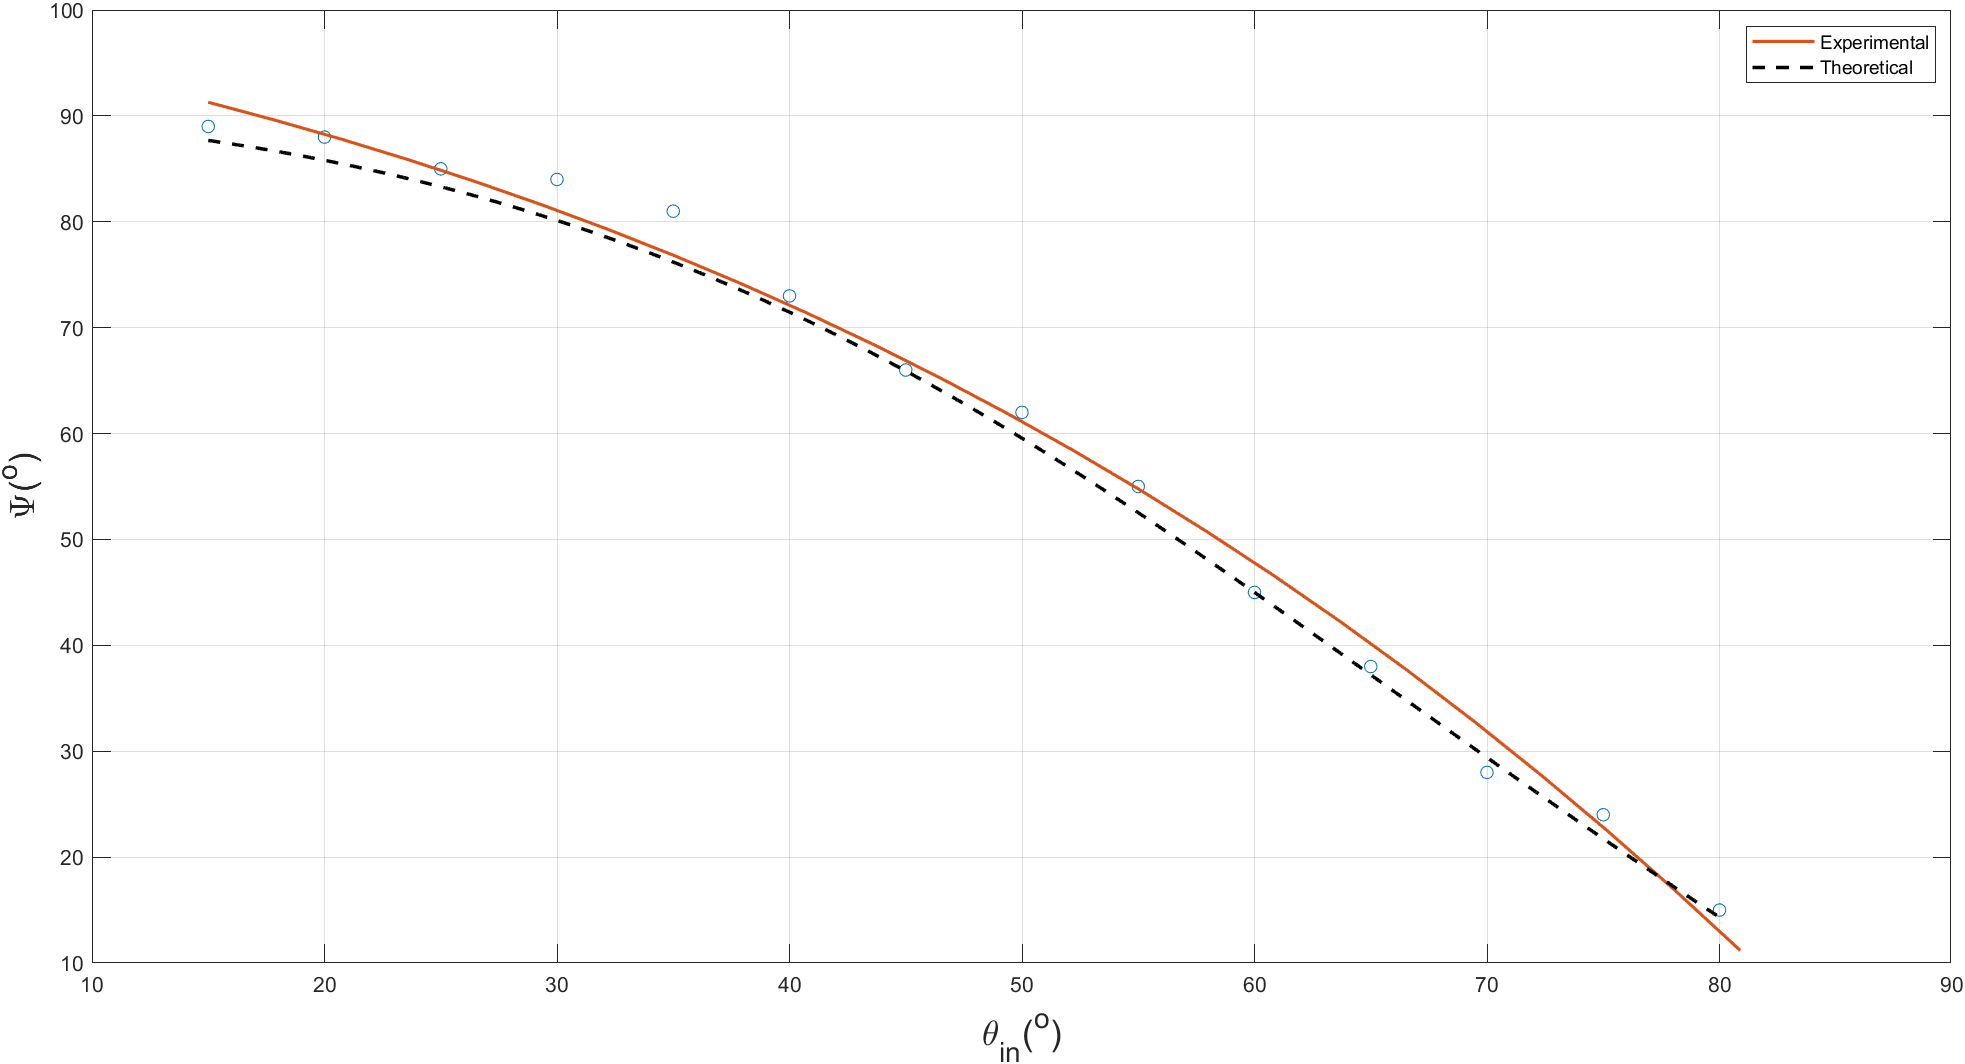
\includegraphics[scale=0.5]{psitheta.png}
\end{figure}

Παρατηρώ πως παρ'όλο που μερικά πειραματικά σημεία απέχουν σημαντικά από τις καμπύλες, η μορφή τους είναι κοινή.

\subsection*{Συμπεράσματα}


Εν τέλει μπορούμε να πούμε πως η άσκηση στα πλαίσια του στόχου της ήταν επιτυχημένη, παρ' όλο που τα αριθμητικά αποτελέσματα δεν ήταν απολύτως συμβατά με τα θεωρητικώς αναμενόμενα. Αυτό διότι ο σκοπός της ήταν να εξετάσουμε την συμπεριφορά της έντασης της ανακλώμενης δέσμης σε σχέση με την πόλωσή της, η οποία είναι εμφνής από τα δύο διαγράμματα. 

Ακόμη, κρίνω πως η κυριότερη πηγή σφάλματος ήταν η τιμή του δείκτη διάθλασης που απείχε και στις δύο περιπτώσεις $\sim 11\%$ από την θεωρητική. Άρα ο προσδιορισμός της γωνίας Brewster στο πρώτο μέρος και της $\theta_{in}$ για την οποία έχουμε $\Psi=45^o$ στο δεύτερο μέρος ίσως να είχαν μεγάλο σφάλμα. Εφόσον παρατηρήθηκε το ίδιο είδους λάθος και στα δύο μέρη, ενδεχομένως να μην είχαμε ορίσει ορθώς το σημείο 0 στο γωνιόμετρο ή να το μετακινήσαμε ακουσίως κατά την διάρκεια του πειράματος.



\end{document}